\documentclass[a4paper,12pt]{article}

\usepackage[utf8]{inputenc}
\usepackage{geometry}

\geometry{
    left=1cm,
    right=1cm,
    top=1.5cm,
    bottom=2.5cm
}

\usepackage{setspace}
\usepackage{tikz}
\usetikzlibrary{trees}

\begin{document}
 
\pagenumbering{arabic}

\begin{Large}
    \begin{singlespace}
       \begin{center}
        \textbf{Red-Black-Tree - Template} \\
        Version 1.0.0
       \end{center} 
    \end{singlespace}
\end{Large}

\vspace*{10mm}

\begin{center}
    
    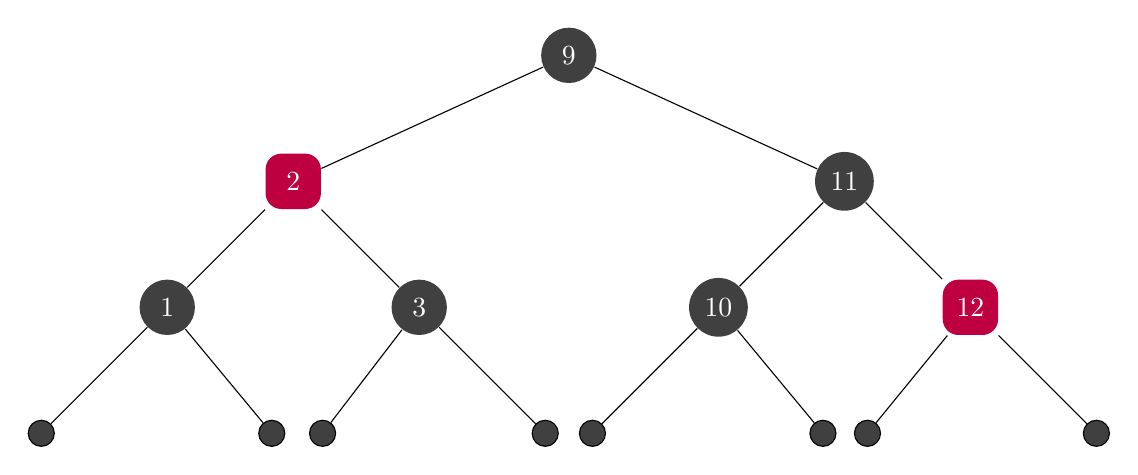
\begin{tikzpicture}[level distance=1.6cm,
        level 1/.style={sibling distance=7cm},
        level 2/.style={sibling distance=3.2cm},
        node distance=1.5cm,
        blackNode/.style = {shape=circle,fill=darkgray,text=white,minimum size=2em},
        redNode/.style = {fill=purple,text=white,rounded corners=2mm,minimum size=2em},
        endNode/.style = {shape=circle,draw=black,fill=darkgray,text=white}
        ]
        \node[blackNode] {9}
        child {node[redNode] {2} 
        child {node[blackNode] {1}
        child{node[endNode] {}}
        child{node[left=1mm][endNode] {}}}
        child {node[blackNode] {3}
        child{node[right=2mm][endNode] {}}
        child{node[endNode] {}}}}
        child {node[blackNode] {11} 
        child {node[blackNode] {10} 
        child {node[endNode] {}} 
        child {node[left=1mm][endNode] {}}} 
        child {node[redNode] {12} 
        child {node[right=1.2mm][endNode] {}} 
        child {node[endNode] {}}}};
    \end{tikzpicture}
\end{center}
    
\end{document}